\documentclass[11pt]{article}

% ---------------------------------------------------------------
% Packages
% ---------------------------------------------------------------
\usepackage[T1]{fontenc}
\usepackage[utf8]{inputenc}
\usepackage{lmodern}
\usepackage[margin=1in]{geometry}
\usepackage{amsmath,amssymb}
\usepackage{enumitem}
\usepackage{xcolor}
\usepackage{tikz}
\usetikzlibrary{positioning,arrows.meta,shapes.geometric}
\usepackage{caption}
\usepackage{float}
\usepackage[hidelinks]{hyperref}

\setlist{itemsep=2pt,topsep=4pt}

\definecolor{accent}{HTML}{2F6DB5}
\definecolor{okgreen}{HTML}{2E7D32}
\definecolor{warnamber}{HTML}{B7791F}
\definecolor{badred}{HTML}{C62828}

\newcommand{\verified}{\textcolor{okgreen}{\textbf{[verified]}}}
\newcommand{\unverified}{\textcolor{warnamber}{\textbf{[unverified]}}}
\newcommand{\contradicted}{\textcolor{badred}{\textbf{[contradicted]}}}

% ---------------------------------------------------------------
\title{\textbf{Software Licensing Explainability with LLMs}\\[4pt]
\large ENSF 621 --- Simplified Design (v1)}
\author{Team Member Name(s)}
\date{\today}

\begin{document}
\maketitle

\noindent
Version 1 (v1) is a deliberately small version of the full design. It keeps the core idea --- recommend an open-source license and explain it faithfully --- and reduces the pipeline to \textbf{two models: a Large Language Model (LLM) and a Natural Language Inference (NLI) model}. Retrieval, a rules engine, repository scanning, and fine-tuned classifiers are deferred to v2.

% ===============================================================
\section{Objectives}
% ===============================================================

\textbf{Primary objective:} build and evaluate a two-stage LLM + NLI pipeline that takes a project description or a dependency manifest, recommends suitable open-source licenses, and explains each recommendation with claims that are automatically checked against the license text.

\begin{description}[leftmargin=1.2cm,style=nextline]
  \item[O1] \textbf{Understand the input.} Accept either a free-text project description or a dependency manifest (\texttt{requirements.txt}, \texttt{package.json}), and turn it into what the developer needs from a license.
  \item[O2] \textbf{Recommend licenses.} Use an LLM to produce a ranked shortlist (top three) of licenses that fit the description and are compatible with the dependencies.
  \item[O3] \textbf{Explain with evidence.} For each recommendation, have the LLM write short claims, each paired with a quoted clause from the official license text.
  \item[O4] \textbf{Verify every claim.} Use an NLI model to check that each quoted clause supports its claim, and label claims as \emph{verified}, \emph{unverified}, or \emph{contradicted}.
  \item[O5] \textbf{Evaluate without domain experts.} Measure recommendation correctness and explanation faithfulness using public, machine-readable license data as ground truth.
\end{description}

% ===============================================================
\section{Scope}
% ===============================================================

\subsection{Problem Statement}

\begin{quote}
\itshape
Given either a developer's natural-language project description or a dependency manifest, recommend up to three open-source licenses and explain each one with claims that are verified against the license text.
\end{quote}

\subsection{In Scope}

\begin{itemize}
  \item \textbf{Input:} one of the following (both may be given together, in which case the manifest adds dependency constraints to the description):
  \begin{itemize}
    \item a free-text description (e.g., ``I'm building a SaaS library and want improvements to come back to the community'');
    \item a manifest file: \texttt{requirements.txt} (Python) or \texttt{package.json} (npm).
  \end{itemize}
  \item \textbf{Licenses:} the OSI-approved software licenses listed on choosealicense.com ($\approx$40), identified by SPDX IDs.
  \item \textbf{Dependency licenses:} read from registry metadata (PyPI JSON API, npm registry) and normalized to SPDX IDs. Unknown or missing licenses are flagged, not guessed.
  \item \textbf{Output:} up to three ranked licenses, each with verified claims and any compatibility warnings.
\end{itemize}

\subsection{Out of Scope for v1 (Planned for v2)}

\begin{itemize}
  \item Retrieval (RAG), vector store, and rerankers.
  \item A deterministic rules engine or compatibility matrix inside the pipeline (the OSADL matrix is still used for \emph{evaluation}).
  \item Scanning a whole repository by URL, or detecting licenses from source files (ScanCode).
  \item Fine-tuned clause classifiers.
  \item Command-line tool or GitHub Action.
  \item Legal advice, non-software licenses, and jurisdiction-specific interpretation (out of scope in every version).
\end{itemize}

\subsection{Location of the Problem}

\begin{itemize}
  \item \textbf{Jurisdiction:} jurisdiction-neutral. The tool explains what the license text says, not how courts in a given country interpret it.
  \item \textbf{Workflow point:} when a developer is choosing a license for a new project, or checking one against the dependencies they already use.
\end{itemize}

% ===============================================================
\section{System Design}
% ===============================================================

\subsection{Software Architecture}

Figure~\ref{fig:arch} shows the v1 pipeline.

\begin{figure}[H]
\centering
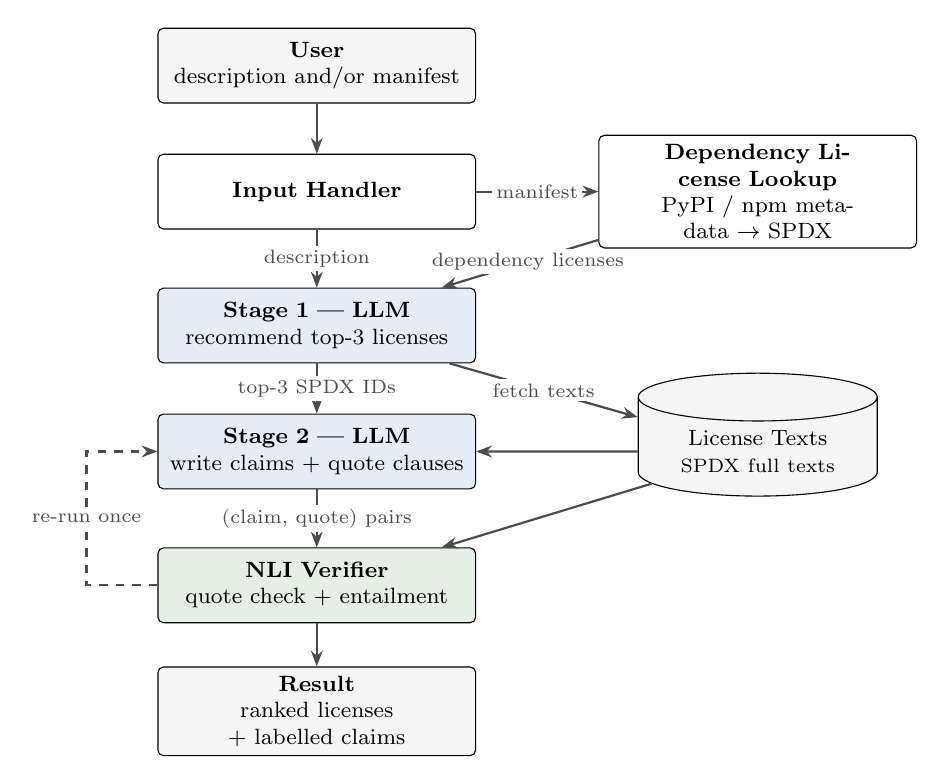
\begin{tikzpicture}[
    font=\footnotesize,
    box/.style={draw, rounded corners=2pt, fill=white, align=center,
                text width=3.8cm, minimum height=0.95cm},
    llm/.style={box, fill=accent!12},
    nli/.style={box, fill=okgreen!12},
    db/.style={draw, cylinder, shape border rotate=90, aspect=0.2,
               fill=black!4, align=center, text width=2.8cm, minimum height=1.2cm},
    arr/.style={-{Stealth[length=2mm]}, thick, black!70},
    tag/.style={font=\scriptsize, fill=white, inner sep=1.5pt},
  ]

  \node[box, fill=black!4] (user) at (0,0)     {\textbf{User}\\description and/or manifest};
  \node[box]               (in)   at (0,-1.6)  {\textbf{Input Handler}};
  \node[box]               (dl)   at (5.6,-1.6){\textbf{Dependency License Lookup}\\PyPI / npm metadata $\rightarrow$ SPDX};
  \node[llm]               (s1)   at (0,-3.3)  {\textbf{Stage 1 --- LLM}\\recommend top-3 licenses};
  \node[db]                (lt)   at (5.6,-4.9){License Texts\\{\scriptsize SPDX full texts}};
  \node[llm]               (s2)   at (0,-4.9)  {\textbf{Stage 2 --- LLM}\\write claims + quote clauses};
  \node[nli]               (v)    at (0,-6.6)  {\textbf{NLI Verifier}\\quote check + entailment};
  \node[box, fill=black!4] (out)  at (0,-8.2)  {\textbf{Result}\\ranked licenses + labelled claims};

  \draw[arr] (user) -- (in);
  \draw[arr] (in) -- node[tag] {manifest} (dl);
  \draw[arr] (in) -- node[tag] {description} (s1);
  \draw[arr] (dl) -- node[tag, pos=0.45] {dependency licenses} (s1);
  \draw[arr] (s1) -- node[tag] {top-3 SPDX IDs} (s2);
  \draw[arr] (s1) -- node[tag, pos=0.5] {fetch texts} (lt);
  \draw[arr] (lt) -- (s2);
  \draw[arr] (lt) -- (v);
  \draw[arr] (s2) -- node[tag] {(claim, quote) pairs} (v);
  \draw[arr] (v) -- (out);
  \draw[arr, dashed] (v.west) -- ++(-0.9,0) |- node[tag, pos=0.25] {re-run once} (s2.west);
\end{tikzpicture}
\caption{v1 architecture. Two LLM stages produce the recommendation and the evidence-backed claims; the NLI verifier checks each claim against the official license text.}
\label{fig:arch}
\end{figure}

\paragraph{Components.}
\begin{enumerate}
  \item \textbf{Input Handler:} accepts the description and/or manifest file and validates it.
  \item \textbf{Dependency License Lookup} (manifest only, not ML): parses the manifest, queries PyPI/npm for each package's declared license, and maps it to an SPDX ID. Packages with missing or ambiguous license information are marked \emph{unknown}.
  \item \textbf{Stage 1 --- Recommendation (LLM):} given the description and the list of dependency licenses, the LLM returns structured JSON containing the developer's inferred requirements, the top three licenses with a short reason for each, and any dependency conflicts it identifies.
  \item \textbf{License Texts:} the official SPDX full texts of the recommended licenses (and of any dependency licenses involved in a conflict). This is a plain file lookup, not a vector database.
  \item \textbf{Stage 2 --- Explanation (LLM):} given the license texts, the LLM writes three to five plain-language claims per license. Each claim must include a \emph{verbatim quote} from the license text as evidence.
  \item \textbf{NLI Verifier:} for each (quote, claim) pair:
  \begin{itemize}
    \item \textbf{Quote check:} confirm that the quote appears verbatim in the SPDX text. If it does not, the claim is \emph{unverified}.
    \item \textbf{Entailment check:} run the NLI model with the quote as the premise and the claim as the hypothesis. Entailment $\rightarrow$ \emph{verified}; contradiction $\rightarrow$ \emph{contradicted}; neutral $\rightarrow$ \emph{unverified}.
    \item If too many claims fail, Stage 2 is re-run once with the failed claims pointed out.
  \end{itemize}
  \item \textbf{Result:} ranked licenses with each claim labelled, plus warnings for unknown dependency licenses and possible conflicts.
\end{enumerate}

\paragraph{Why two LLM stages?}
Separating ``pick licenses'' from ``explain them'' means the LLM only receives the full text of the three licenses it chose. This keeps prompts short and gives the LLM exact text to quote from, which the NLI verifier needs.

\paragraph{Technology stack.}
Python, an LLM API (or a local open-weight model), Hugging Face Transformers for NLI, SPDX license-list-data (JSON), and Streamlit for the user interface.

\subsection{Machine Learning Models}

\begin{description}[leftmargin=0pt,style=nextline]
  \item[M1 --- Large Language Model]
  \begin{itemize}
    \item \textbf{Role:} interprets the description, infers requirements, recommends the top three licenses (Stage 1), and writes claims with quoted evidence (Stage 2).
    \item \textbf{Why it is useful:} mapping vague intent (``I don't want big companies taking my code without giving back'') to license concepts such as copyleft or network clauses requires language understanding that rules cannot provide. It also turns legal text into readable explanations.
    \item \textbf{Candidates:} a hosted model (e.g., Claude Sonnet 5) and one open-weight model (e.g., Llama or Qwen, 7--8B), so the two can be compared.
    \item \textbf{Output format:} schema-constrained JSON, so every stage can be parsed and evaluated automatically.
  \end{itemize}

  \item[M2 --- Natural Language Inference (NLI) Model]
  \begin{itemize}
    \item \textbf{Role:} checks whether each quoted license clause entails the claim the LLM made about it.
    \item \textbf{Why it is useful:} it is an independent check that does not share the LLM's mistakes. It catches claims the license text does not support, and it doubles as an automatic faithfulness metric for evaluation, which matters because no legal expert is available.
    \item \textbf{Candidates:} \texttt{DeBERTa-v3-large-mnli} (primary) and \texttt{roberta-large-mnli} (comparison).
  \end{itemize}
\end{description}

% ===============================================================
\section{Evaluation}
% ===============================================================

All ground truth comes from public, curated sources.

\begin{description}[leftmargin=0pt,style=nextline]
  \item[Recommendation from a description]
  \begin{itemize}
    \item \textbf{Ground truth:} requirement profiles built from choosealicense.com's permission, condition, and limitation labels. The correct answer set is every license whose labels match the profile. An LLM writes natural-language descriptions for each profile, and the team spot-checks a sample.
    \item \textbf{Metrics:} Hit@1, Hit@3, and the percentage of recommendations that violate a stated requirement.
  \end{itemize}

  \item[Recommendation from a manifest]
  \begin{itemize}
    \item \textbf{Ground truth:} real dependency sets from PyPI/npm packages. Correct answers are licenses that the OSADL compatibility matrix marks as compatible with every dependency.
    \item \textbf{Metrics:} percentage of incompatible recommendations and percentage of conflicts correctly flagged.
  \end{itemize}

  \item[Explanation faithfulness]
  \begin{itemize}
    \item \textbf{Ground truth:} the SPDX license text itself.
    \item \textbf{Metrics:} percentage of quotes found verbatim, percentage of claims entailed, and percentage contradicted.
  \end{itemize}

  \item[Effect of the verifier]
  \begin{itemize}
    \item \textbf{Method:} compare LLM-only output with LLM + NLI output.
    \item \textbf{Metric:} reduction in unsupported claims shown to the user.
  \end{itemize}

  \item[Reliability of the NLI verifier]
  \begin{itemize}
    \item \textbf{Ground truth:} about 100--150 claim/clause pairs hand-labelled by the team, plus \emph{automatically generated negatives}: true claims derived from choosealicense.com labels (e.g., ``you must disclose source'') and their negations (e.g., ``you do not need to disclose source''), each paired with the relevant clause.
    \item \textbf{Metrics:} precision, recall, and F1 of the NLI model against these labels.
  \end{itemize}
\end{description}

\paragraph{Baselines.}
\begin{itemize}
  \item LLM-only (Stage 1 + Stage 2, no verifier).
  \item Hosted LLM versus open-weight LLM, both with the verifier.
\end{itemize}

\paragraph{Small human check.}
Ten to fifteen classmates rate explanation clarity and answer a few comprehension questions (e.g., ``Can you use this in closed-source software?''), scored against the choosealicense.com labels.

% ===============================================================
\section{User Interface}
% ===============================================================

v1 is a single-page \textbf{Streamlit} application.

\begin{itemize}
  \item \textbf{Input panel:} two tabs, \emph{Describe your project} (text box) and \emph{Upload manifest} (file upload for \texttt{requirements.txt} or \texttt{package.json}). Both can be filled in.
  \item \textbf{Dependency list} (when a manifest is uploaded): each package with its license and a status of compatible, unknown, or possible conflict.
  \item \textbf{Result cards:} one card per recommended license, showing its rank and a one-line reason; its claims, each with a badge (\verified, \unverified, or \contradicted); and an expandable evidence section with the quoted clause.
  \item \textbf{Footer:} ``Explanations are based on license text only. This is not legal advice.''
\end{itemize}

\begin{figure}[H]
\centering
\fbox{%
\begin{minipage}{0.88\textwidth}
\vspace{4pt}
\textbf{[\,Describe your project\,]} \quad \textcolor{black!50}{[\,Upload manifest\,]}\\[4pt]
\fbox{\begin{minipage}{0.96\textwidth}\small\itshape
SaaS analytics library; improvements should come back to the community.
\end{minipage}}\\[4pt]
\hspace*{\fill}\textcolor{accent}{\textbf{[\,Recommend\,]}}

\vspace{4pt}\hrule\vspace{6pt}
\small
\textbf{1. AGPL-3.0} --- covers use over a network\\[2pt]
\hspace*{1em}\verified\ Network users must be offered the source code. \hfill \textcolor{accent}{show quote}\\
\hspace*{1em}\verified\ Modified versions must remain under AGPL-3.0. \hfill \textcolor{accent}{show quote}\\
\hspace*{1em}\unverified\ Compatible with all your dependencies. \hfill \textcolor{accent}{show quote}\\[4pt]
\textbf{2. GPL-3.0} --- strong copyleft, no network clause\\[2pt]
\textbf{3. MPL-2.0} --- file-level copyleft

\vspace{6pt}\hrule\vspace{4pt}
{\footnotesize\textcolor{black!60}{Explanations are based on license text only. This is not legal advice.}}
\vspace{2pt}
\end{minipage}}
\caption{Mock-up of the v1 Streamlit interface.}
\label{fig:ui}
\end{figure}

% ===============================================================
\section{From v1 to v2}
% ===============================================================

v2 extends v1 as follows:

\begin{itemize}
  \item \textbf{Recommendation:} the LLM picking licenses is replaced by a deterministic rules engine and the OSADL compatibility matrix deciding the facts, with the LLM only explaining.
  \item \textbf{Evidence:} passing the full text of three licenses to the LLM is replaced by retrieval (embeddings and a reranker) over clause chunks.
  \item \textbf{Dependencies:} registry metadata is supplemented by ScanCode license detection and repository URL scanning.
  \item \textbf{Verification:} the NLI verifier is joined by a fine-tuned clause classifier for modified or unknown licenses.
  \item \textbf{Interface:} the Streamlit page grows into a full web application with a command-line tool / GitHub Action.
\end{itemize}

v1's evaluation results --- especially how often the LLM alone recommends incompatible licenses --- will show whether building the v2 rules engine is worthwhile.

\end{document}
